\documentclass{article}
\usepackage[utf8]{inputenc}
\usepackage{amssymb}
\usepackage{tikz}
\usepackage{amsmath}
\usepackage{relsize}
\usepackage{mathtools}
\usepackage{textcomp}
\usepackage{eurosym}
\usepackage{amssymb}
\usepackage{systeme}
\usepackage{mathtools}

\title{Results}
\author{Roman Oort}
\date{\today}

%%% PERSONAL SHORTCUTS
\DeclareMathOperator*{\plim}{plim}
\newcommand{\T}{\textbf{T}}
\newcommand{\Tij}{\textbf{T}_{ij}}
\newcommand{\Soc}{(\T(n))^{\infty}_{n=1}}
\newcommand{\beli}[3][2]{p_{#2}^{(#3)}}
\newcommand{\belvec}[2]{\textbf{p}^{(#2)}}

\begin{document}

\maketitle

\tableofcontents
\newpage
\section{Results}

All results obtained and discussed in the following section are generated with an identical network structure, unless mentioned otherwise. The networks used are all directed networks, with an increased degree, using the default distribution for the degree increase. Furthermore, the probability of a self-link is $1$, meaning that every agent will have a link to itself. Finally, uniform weight initialization was applied.

\subsection{Cooperative Networks}

\begin{center}\todo{increase font-size}
    \begin{figure}[!htbp]
        \centering
        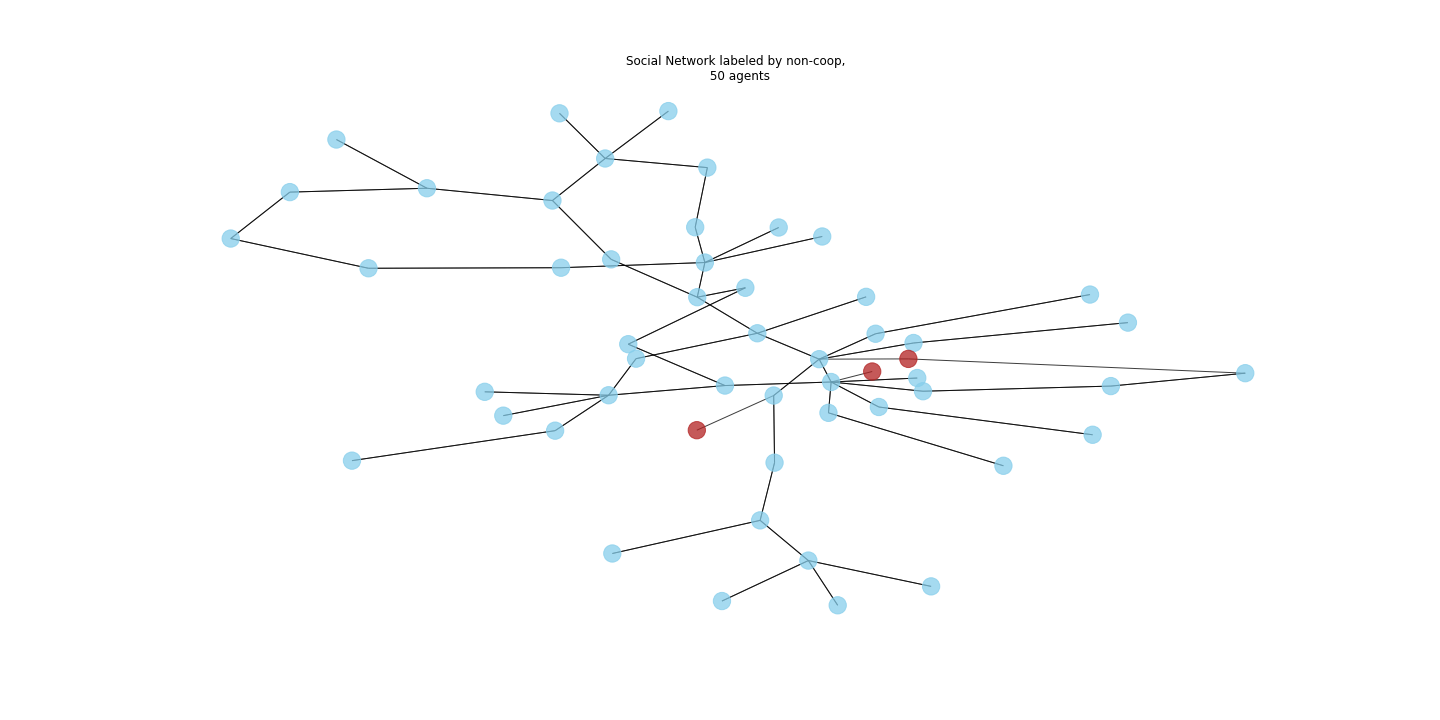
\includegraphics[width=1\textwidth]{ThesisKI/Images/NonCoopGraph.png}
        \caption{Non-cooperative network, $n=50, m=3$}
        \label{network:noncoop}
    \end{figure}
\end{center}

\subsection{Non-cooperative networks, $n=1$}

\subsection{Non-cooperative networks, $n > 1$}

\end{document}